\section{Introdução à lógica}

\begin{frame}{Princípios de resolução de problemas}
    \fontsize{12pt}{15}\selectfont{
    Primeiramente é preciso entender e compreender a palavra ``problema''. Pode-se dizer que problema é uma proposta duvidosa, que pode ter numerosas soluções, ou questão não resolvida e que é objetivo de discussão.
        
	}\par
	\vspace{1em}
\end{frame}


\begin{frame}{Princípios de resolução de problemas}
    \fontsize{12pt}{15}\selectfont{
    Problema é uma questão que foge a uma determinada regra, ou melhor, é o desvio de um percurso, o qual impede de atingir um determinado objetivo com eficiência e eficácia.
        
	}\par
	\vspace{1em}
\end{frame}

\begin{frame}{Princípios de resolução de problemas}
    \fontsize{12pt}{15}\selectfont{
    Os diagramas de blocos são realmente um bom instrumento para avaliação do problema do fluxo de informações de um dado sistema. Por esse motivo deve-se resolver um problema de lógica usando um procedimento de desenvolvimento.
	}\par
	\vspace{1em}
\end{frame}


\begin{frame}{Princípios de resolução de problemas}
    \fontsize{12pt}{15}\selectfont{
    Princípios para uso do diagrama de blocos:
	}\par
	\vspace{0.5cm}
	\begin{enumerate}
	    \item Os diagramas de blocos devem ser feitos e quebrados em vários níveis. Os primeiros diagramas devem conter apenas as ideias gerais, deixando para as etapas posteriores os demais detalhamentos.
	    
	    \item Para o desenvolvimento correto de um diagrama de bloco, ele deve ser iniciado de cima para baixo.
	    
	    \item É incorreto e ``proibido'' ocorrer o cruzamento de linhas de fluxo de dados entre os símbolos.
	\end{enumerate}
	\vspace{1em}
\end{frame}


\begin{frame}{Exemplo}
    \fontsize{12pt}{15}\selectfont{
    Uma faculdade qualquer, cujo cálculo da média é realizado com três notas que determinam a aprovação ou reprovação dos seus alunos. Há pesos diferentes para as notas, as duas primeiras notas tem peso 4, logo a última tem peso 2. Considere ainda que o valor da média deve ser maior ou igual a 7 para que haja aprovação.
	}\par
	\vspace{1em}
\end{frame}



\begin{frame}{Exemplo}
    \fontsize{12pt}{15}\selectfont{
    Uma faculdade qualquer, cujo cálculo da média é realizado com três notas que determinam a aprovação ou reprovação dos seus alunos. Há pesos diferentes para as notas, as duas primeiras notas tem peso 4, logo a última tem peso 2. Considere ainda que o valor da média (ponderada) deve ser maior ou igual a 7 para que haja aprovação.
	}\par
	\vspace{1em}
	Média final$~=~\frac{Nota1*4 + Nota2 * 4 + Nota3 * 2}{10}$
\end{frame}





\begin{frame}{Exemplo}

\begin{figure}[h!]
    \centering
\begin{tikzpicture}[node distance=1.5cm,thick,scale=1, every node/.style={scale=0.7}]
\centering
\node (start) [startstop] {Início};
\node (pro2a) [process, below of=start] {calcular a média e determinar a aprovação};
    \draw [arrow] (start) -- (pro2a);
\node (stop) [startstop, below of=pro2a] {Fim};
    \draw [arrow] (pro2a) -- (stop);
    
\end{tikzpicture}
\caption{Diagrama de blocos para o cálculo da média.}
\label{flux:fluxograma}
\end{figure}

\end{frame}



\begin{frame}{Exemplo}

\begin{figure}[h!]
    \centering
\begin{tikzpicture}[node distance=1.5cm,thick,scale=1, every node/.style={scale=0.7}]
\centering
\node (start) [startstop] {Início};
\node (ioinicio) [io, below of=start] {Entrada com 3 notas};
    \draw [arrow] (start) -- (ioinicio); 
    
\node (pro2a) [process, below of=ioinicio] {calcular a média e determinar a aprovação};
    \draw [arrow] (ioinicio) -- (pro2a);
    
\node (iofinal) [io, below of=pro2a] {Apresentar se houver ou não aprovação};
    \draw [arrow] (pro2a) -- (iofinal); 
    
\node (stop) [startstop, below of=iofinal] {Fim};
    \draw [arrow] (iofinal) -- (stop);
    
\end{tikzpicture}
\caption{Diagrama de blocos para o cálculo da média.}
\label{flux:fluxograma}
\end{figure}

\end{frame}





\begin{frame}{Exemplo}

\begin{figure}[h!]
    \centering
\begin{tikzpicture}[node distance=1.5cm,thick,scale=1, every node/.style={scale=0.5}]
\centering
\node (start) [startstop] {Início};
\node (ioinicio) [io, below of=start] {Entrada com 3 notas};
    \draw [arrow] (start) -- (ioinicio); 
    
\node (pro2a) [process, below of=ioinicio] {calcular a média};
    \draw [arrow] (ioinicio) -- (pro2a);

\node (dec1)  [decision, below of=pro2a, yshift=-2cm] {Média >= 7};
\node (pro2f) [io, right of=dec1, xshift=7cm] {Apresenta ``Aprovado''};
            \draw [arrow] (pro2a) -- (dec1);
    \draw [arrow] (dec1) -- node[yesnode] {Sim} (pro2f);   % <--- using nodestyle "nonode"

\node (pro2g) [io, below of=dec1, xshift=1cm] {Apresenta ``Reprovado''};
    \draw [arrow] (dec1) -- node[nonode] {Não} (stop);

% \node (dec2)  [decision, below of=dec1, yshift=-3.5cm] {Verificar Exactidão};
    % \draw [arrow] (dec1) -- node[nonode] {Não} (dec2);   % <--- using nodestyle "yesnode"
    %   \draw [arrow] (dec2) -- node[anchor=south] {yes} (stop);
\node (stop) [startstop, below of=pro2f, yshift=-2cm] {Fim};
        \draw [arrow] (pro2f) -- (stop);
        \draw [arrow] (pro2g) -- (stop);
        % \draw [arrow] (dec2) -- node[yesnode] {Sim} (stop);
            % \draw [arrow] (dec2) -| node[nonode] (-1,0) {Não} (pro2f);



% \node (dec1) [decision, below of=pro2a, yshift=-2cm] {Média >= 7};
%     \draw [arrow] (pro2a) -- (dec1);
  
% \node (iofinal) [io, below of=dec1] {Apresentar se houver ou não aprovação};
%     \draw [arrow] (dec1) -- (iofinal); 
%     \draw [arrow] (dec1) -- node[nonode] {Não} (iofinal);   % <--- using nodestyle "nonode"
    
% \node (stop) [startstop, below of=iofinal, yshift=-2cm] {Fim};
%         \draw [arrow] (dec1) -- node[yesnode] {Sim} (stop);
        
% \node (stop) [startstop, below of=iofinal] {Fim};
%     \draw [arrow] (iofinal) -- (stop);
    
\end{tikzpicture}
\caption{Diagrama de blocos para o cálculo da média.}
\label{flux:fluxograma}
\end{figure}

\end{frame}



% \begin{frame}{Exemplo}

% \begin{figure}[h!]
%     \centering
% \begin{tikzpicture}[node distance=1cm,thick,scale=1, every node/.style={scale=0.3}]
% \centering
% \node (start) [startstop] {Início do Processamento};
% \node (pro2a) [process, below of=start] {Definir os Métodos de Solução};
%         \draw [arrow] (start) -- (pro2a);
% \node (pro2b) [process, below of=pro2a] {Definir os Controlos da Solução};
%         \draw [arrow] (pro2a) -- (pro2b);
% \node (pro2c) [process, below of=pro2b] {Definir os Monitores da Solução};
%         \draw [arrow] (pro2b) -- (pro2c);
% \node (pro2d) [process, below of=pro2c] {Inicializar a Simulação};
%         \draw [arrow] (pro2c) -- (pro2d);
% \node (pro2e) [process, below of=pro2d] {Efetuar o cálculo numérico};
%         \draw [arrow] (pro2d) -- (pro2e);
% \node (dec1)  [decision, below of=pro2e, yshift=-2cm] {Verificar convergência};
% \node (pro2f) [process, right of=dec1, xshift=7cm] {Modificar paramêtros da malha ou da Solução};
%             \draw [arrow] (pro2e) -- (dec1);
%     \draw [arrow] (dec1) -- node[nonode] {Não} (pro2f);   % <--- using nodestyle "nonode"
% \node (dec2)  [decision, below of=dec1, yshift=-3.5cm] {Verificar Exactidão};
%     \draw [arrow] (dec1) -- node[yesnode] {Sim} (dec2);   % <--- using nodestyle "yesnode"
%     %   \draw [arrow] (dec2) -- node[anchor=south] {yes} (stop);
% \node (stop) [startstop, below of=dec2, yshift=-2cm] {Fim do Processamento};
%         \draw [arrow] (dec2) -- node[yesnode] {Sim} (stop);
%             \draw [arrow] (dec2) -| node[nonode] (-1,0) {Não} (pro2f);
% %\node (out1) [io, below of=pro2a] {Output};
% \end{tikzpicture}
% % \caption[Propriedades Físicas de um escoamento]{Propriedades Físicas de um escoamento, retirado de \cite{Tu2013}.}
% \label{flux:fluxograma}
% \end{figure}

% \end{frame}







\begin{frame}{Particularidades entre lógicas}
    \fontsize{12pt}{15}\selectfont{
        \begin{itemize}
            \item \textbf{Linear}: a técnica lógica \textbf{linear} é conhecida como um modelo tradicional de desenvolvimento e resolução de um problema.
            
            \item \textbf{Estruturada}: a técnica de lógica \textbf{estruturada} é mais usada pelo profissionais de desenvolvimento de sistemas. Possui características e padrões da técnica de lógica linear.
            
            \item \textbf{Modular}: a técnica da lógica \textbf{modular} é usada decompor um diagrama em partes independentes.
            
            \item \textbf{Linguagem C}: linguagem de programação compilada de propósito geral, estruturada, imperativa, procedural.
        \end{itemize}
	}\par
	\vspace{1em}
\end{frame}



\begin{frame}{Lógica estruturada}
    \fontsize{14pt}{15}\selectfont{
        É uma forma de lógica com ênfase no uso de subrotinas, ciclo de repetição, condicionais e estruturas em bloco.
	}\par
	\vspace{1em}
\end{frame}


\begin{frame}{Lógica estruturada}
    \fontsize{12pt}{15}\selectfont{
        Sequência
	}\par
	\vspace{1em}
	\centering
    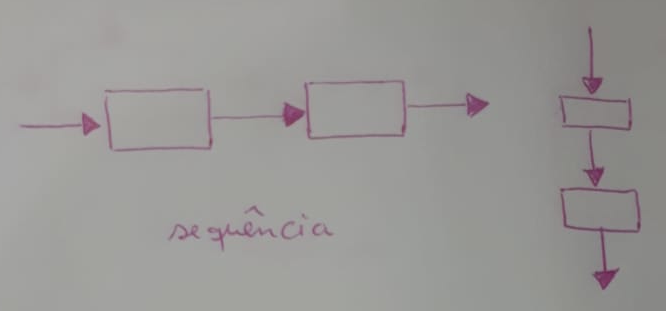
\includegraphics[width=0.7\textwidth]{images/fig-blocos-sequencia.png}
\end{frame}


\begin{frame}{Lógica estruturada}
    \fontsize{12pt}{15}\selectfont{
        Decisão/Condição
	}\par
	\vspace{0.5em}
	\centering
    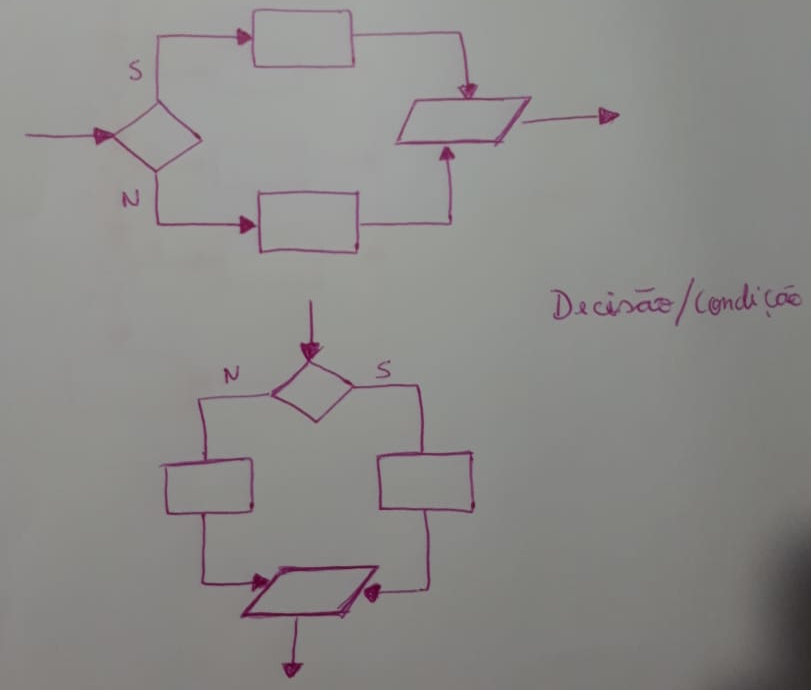
\includegraphics[width=0.6\textwidth]{images/fig-blocos-condicao.png}
\end{frame}


\begin{frame}{Lógica estruturada}
    \fontsize{12pt}{15}\selectfont{
        Repetição
	}\par
	\vspace{1em}
	\centering
    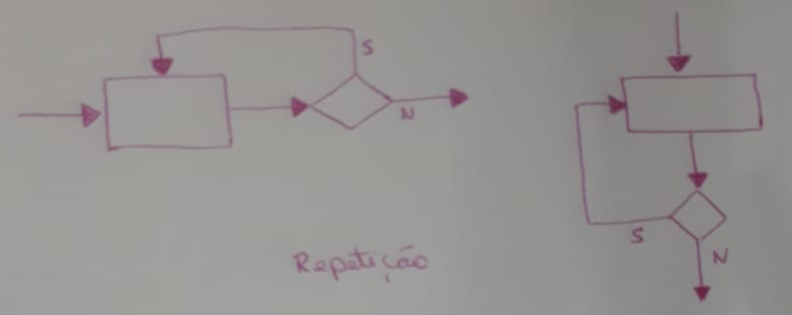
\includegraphics[width=0.7\textwidth]{images/fig-blocos-repeticao.png}
\end{frame}


\begin{frame}{Lógica estruturada}
    \fontsize{12pt}{15}\selectfont{
        Caso
	}\par
	\vspace{1em}
	\centering
    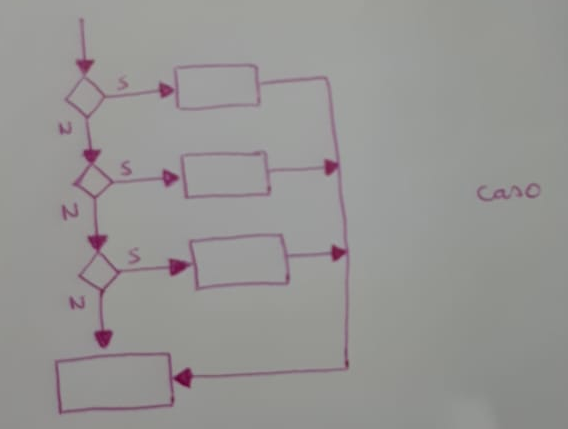
\includegraphics[width=0.6\textwidth]{images/fig-blocos-caso.png}
\end{frame}




\begin{frame}{Lógica Modular}
    \fontsize{12pt}{15}\selectfont{
        A técnica da lógica \textbf{modular} é elaborada como uma estrutura de partes independentes, denominadas de módulos, cujo procedimento segue regras, a saber: 
        
        \vspace{0.5cm}
        
        \begin{itemize}
            \item decompor um diagrama em partes independentes; e
            \item dividir um problema em outros menores.
        \end{itemize}
	}\par
	\vspace{1em}
\end{frame}


\begin{frame}{Lógica modular}
	\vspace{1em}
	\centering
    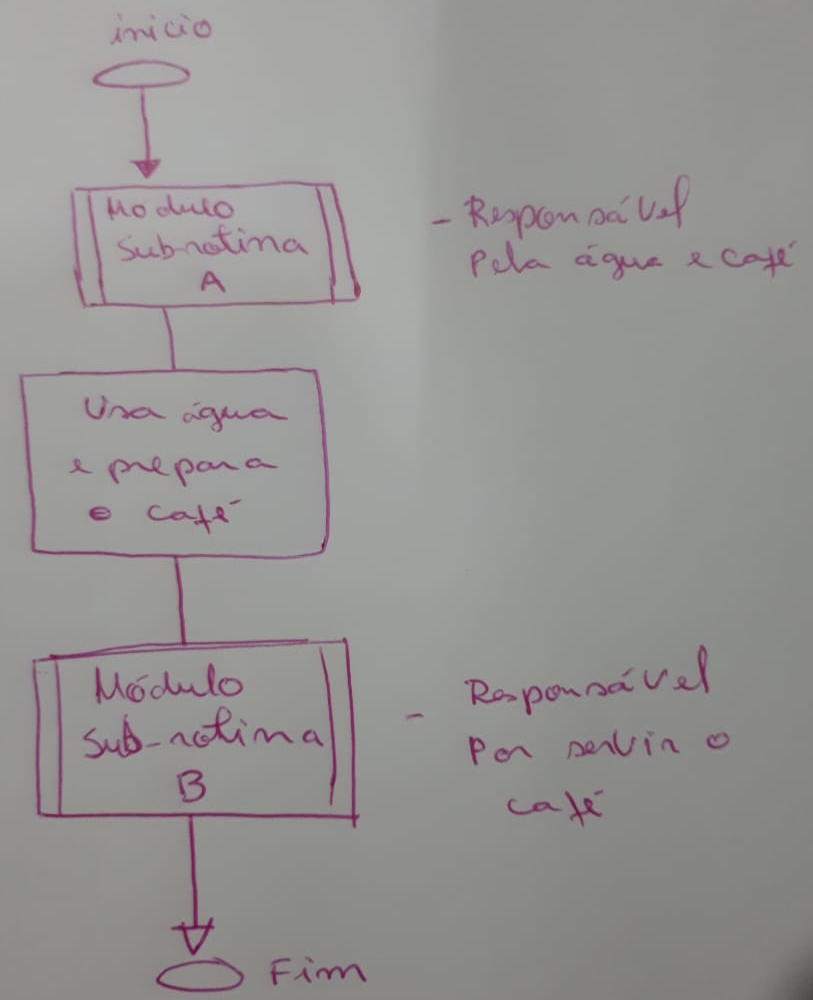
\includegraphics[width=0.45\textwidth]{images/fig-logica-modular.png}
\end{frame}


\begin{frame}{Exercício Lista 2 - Questão 5}
    \fontsize{12pt}{15}\selectfont{
        l2-q5) Utilize diagrama de blocos para resolver o seguir problema: leia três números inteiros e calcule a soma. Considerar que a condição, se a soma for maior que 10, escreva ``tem erro'', do contrário escreva o valor da soma.
	}\par
	\vspace{1em}
\end{frame}

\begin{frame}{Exercício Lista 2 - Questão 5}
	\vspace{1em}
	\centering
    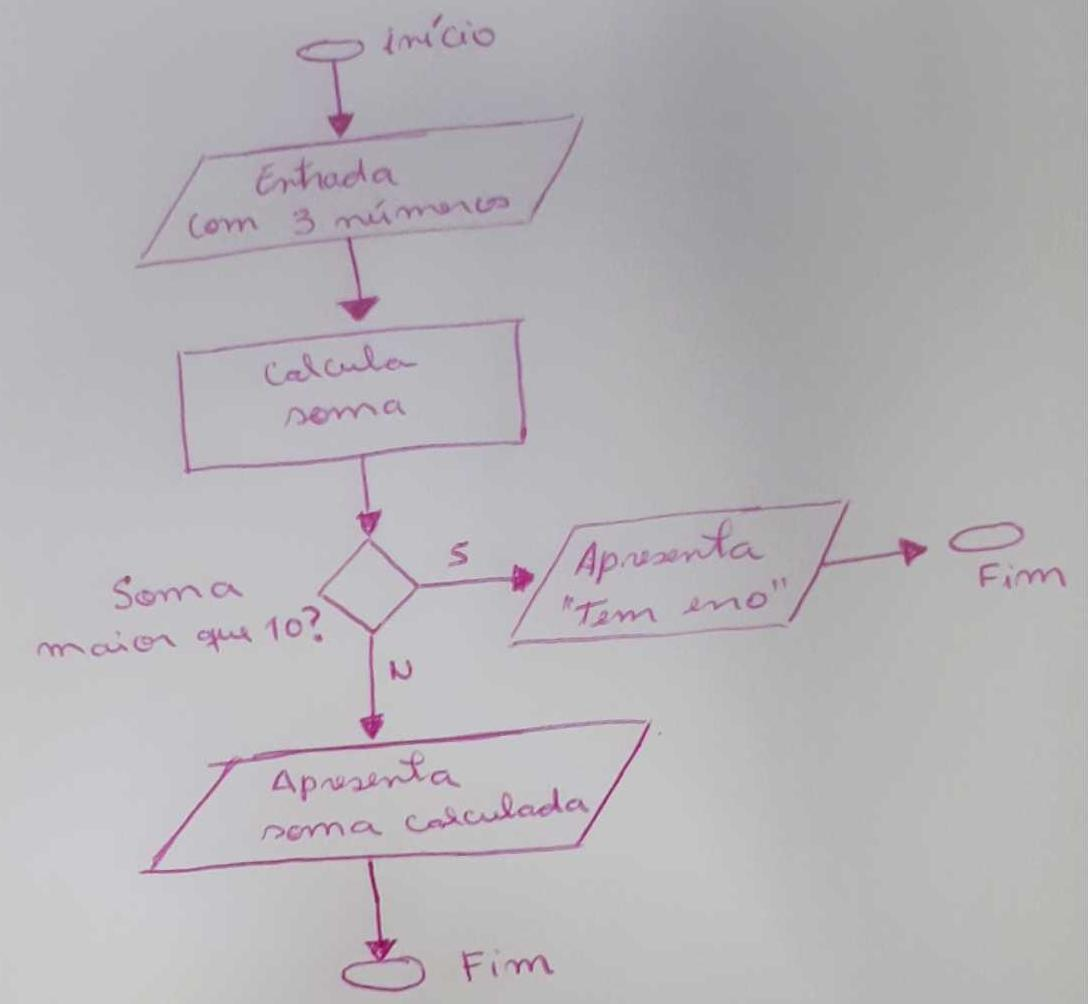
\includegraphics[width=0.55\textwidth]{images/fig-exercicio-02-q5.jpeg}
\end{frame}



\begin{frame}{Exercício Lista 2 - Questão 6}
    \fontsize{12pt}{15}\selectfont{
        l2-q6) Utilize diagrama de blocos para resolver o seguir problema: leia três notas de um aluno, calcule e escreva a média final deste aluno. Considerar que a média é ponderada e que o peso das notas é 2, 3 e 5. 
        \vspace{1cm}
        
        Média Final (MF)~=~$\frac{N1\times 2 + N2 \times 3 + N3 \times 5}{10}$
	}\par
	\vspace{1em}
\end{frame}

\begin{frame}{Exercício Lista 2 - Questão 6}
	\vspace{1em}
	\centering
    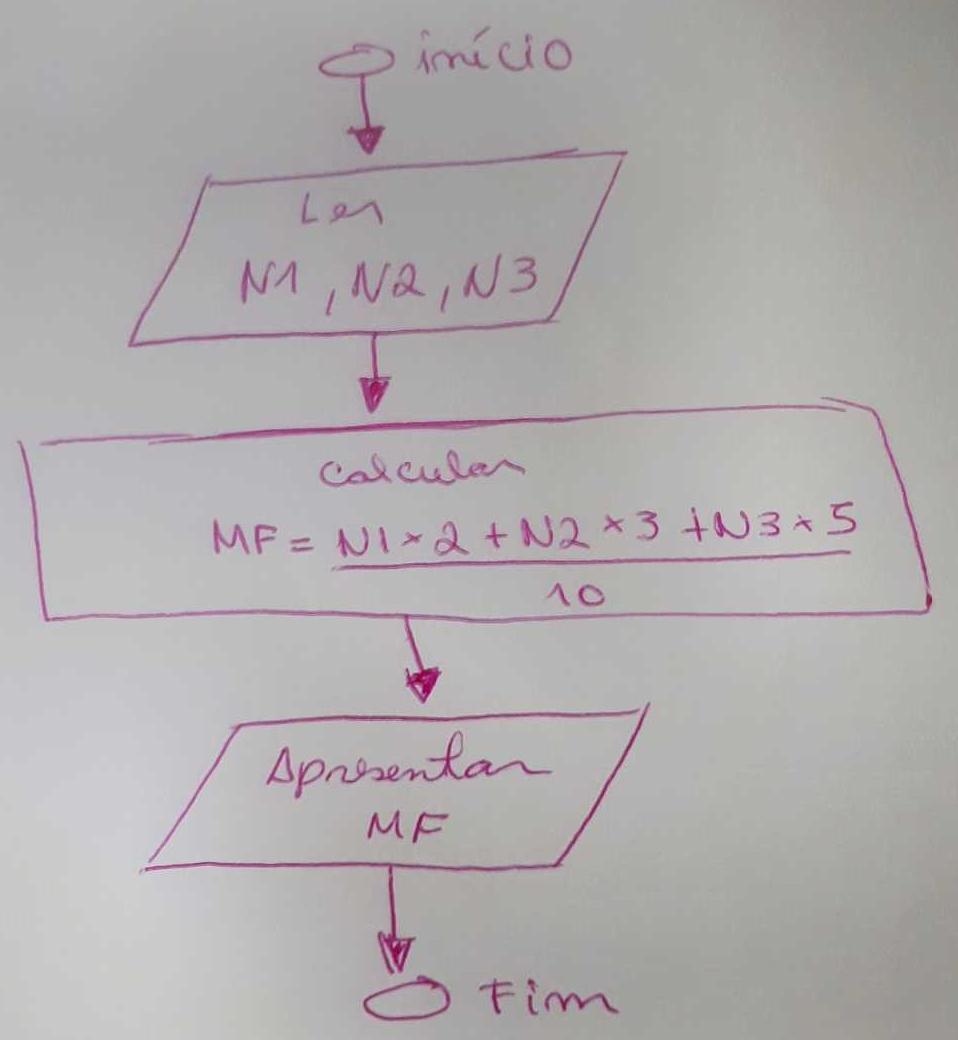
\includegraphics[width=0.5\textwidth]{images/fig-exercicio-02-q6.jpeg}
\end{frame}


\begin{frame}{Exercício Lista 2 - Questão 7}
    \fontsize{12pt}{15}\selectfont{
        l2-q7) Utilize diagrama de blocos para resolver o seguir problema: as maçãs custam R\$ 1,50 cada se forem compradas menos de uma dúzia, e R\$ 1,00 se forem compradas pelo menos 12. leia o número de maçãs compradas, calcule e escreva o custo total da compra. 
        \vspace{1cm}
	}\par
	\vspace{1em}
\end{frame}

\begin{frame}{Exercício Lista 2 - Questão 7}
	\vspace{1em}
	\centering
    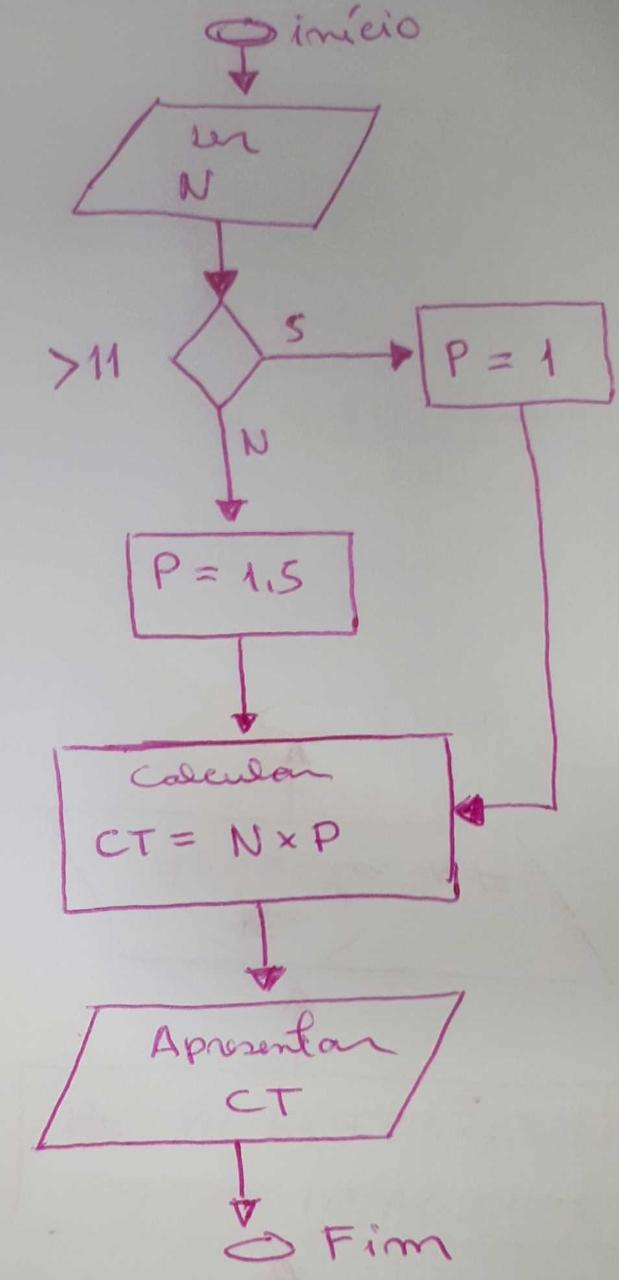
\includegraphics[width=0.3\textwidth]{images/fig-exercicio-02-q7.jpeg}
\end{frame}


\begin{frame}{Exercício Lista 2 - Questão 8}
    \fontsize{12pt}{15}\selectfont{
        l2-q8) Utilize diagrama de blocos para resolver o seguir problema: a jornada de trabalho semanal de um funcionário é de 40 horas. O funcionário que trabalhar mais de 40 horas receberá hora extra, cujo cálculo é o valor da hora regular com um acréscimo de 50\%. leia o número de horas trabalhadas em um mês, o salário por hora e escreva o salário total do funcionário, que deverá ser acrescido das horas extras, caso tenham sido trabalhadas (considere que o mês possua 4 semanas exatas).
        \vspace{1cm}
	}\par
	\vspace{1em}
\end{frame}

\begin{frame}{Exercício Lista 2 - Questão 8}
	\vspace{1em}
	\centering
    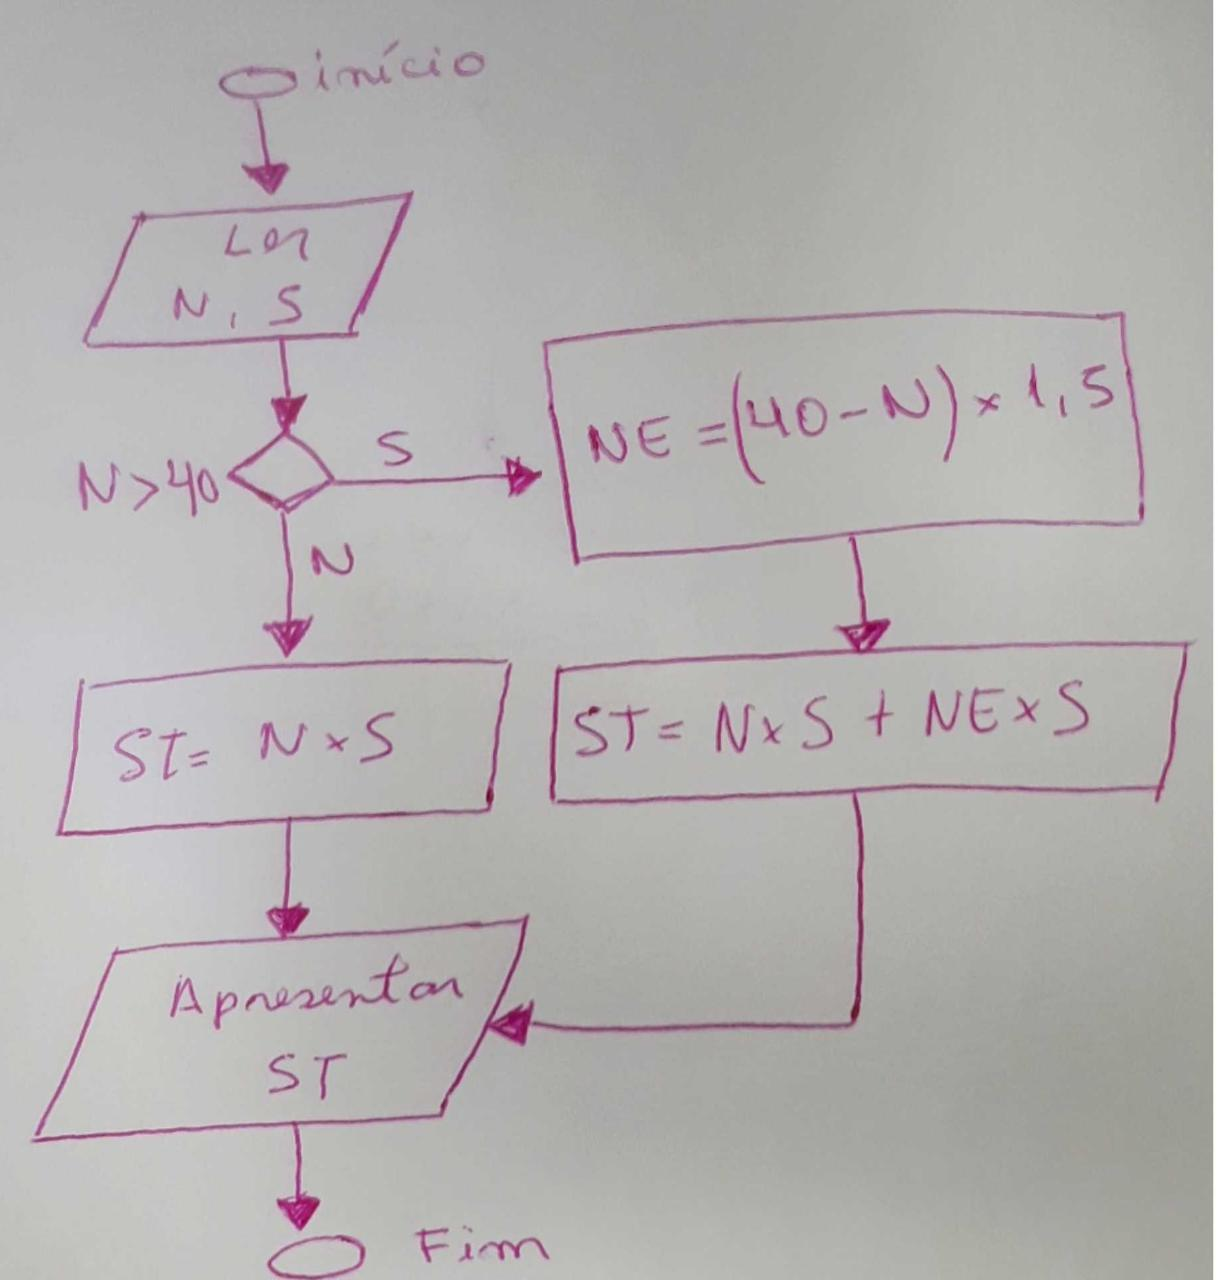
\includegraphics[width=0.5\textwidth]{images/fig-exercicio-02-q8.jpeg}
\end{frame}


